
%==========================================================================

\begin{frame}[fragile]

        {\Huge New Documentation Website}

  \vspace{-20pt}

\end{frame}

%==========================================================================

\begin{frame}[fragile]{Transition to github.io}
\textbf{Kokkos Documentation Now on \url{https://kokkos.github.io}}

\begin{itemize}
  \item {Transition to Sphinx syntax}
  \item {More flexibility in site layout and style}
  \item {Better update processes}
  \begin{itemize}
    \item {Source for core documentaiton at \url{https://github.com/kokkos/kokkos-core-wiki}}
    \item {Using pull requests with auto deploy}
    \item {Pull requests to improvde documentation are welcome!}
  \end{itemize}
\end{itemize}
\end{frame}

\begin{frame}[fragile]{Transition to github.io}
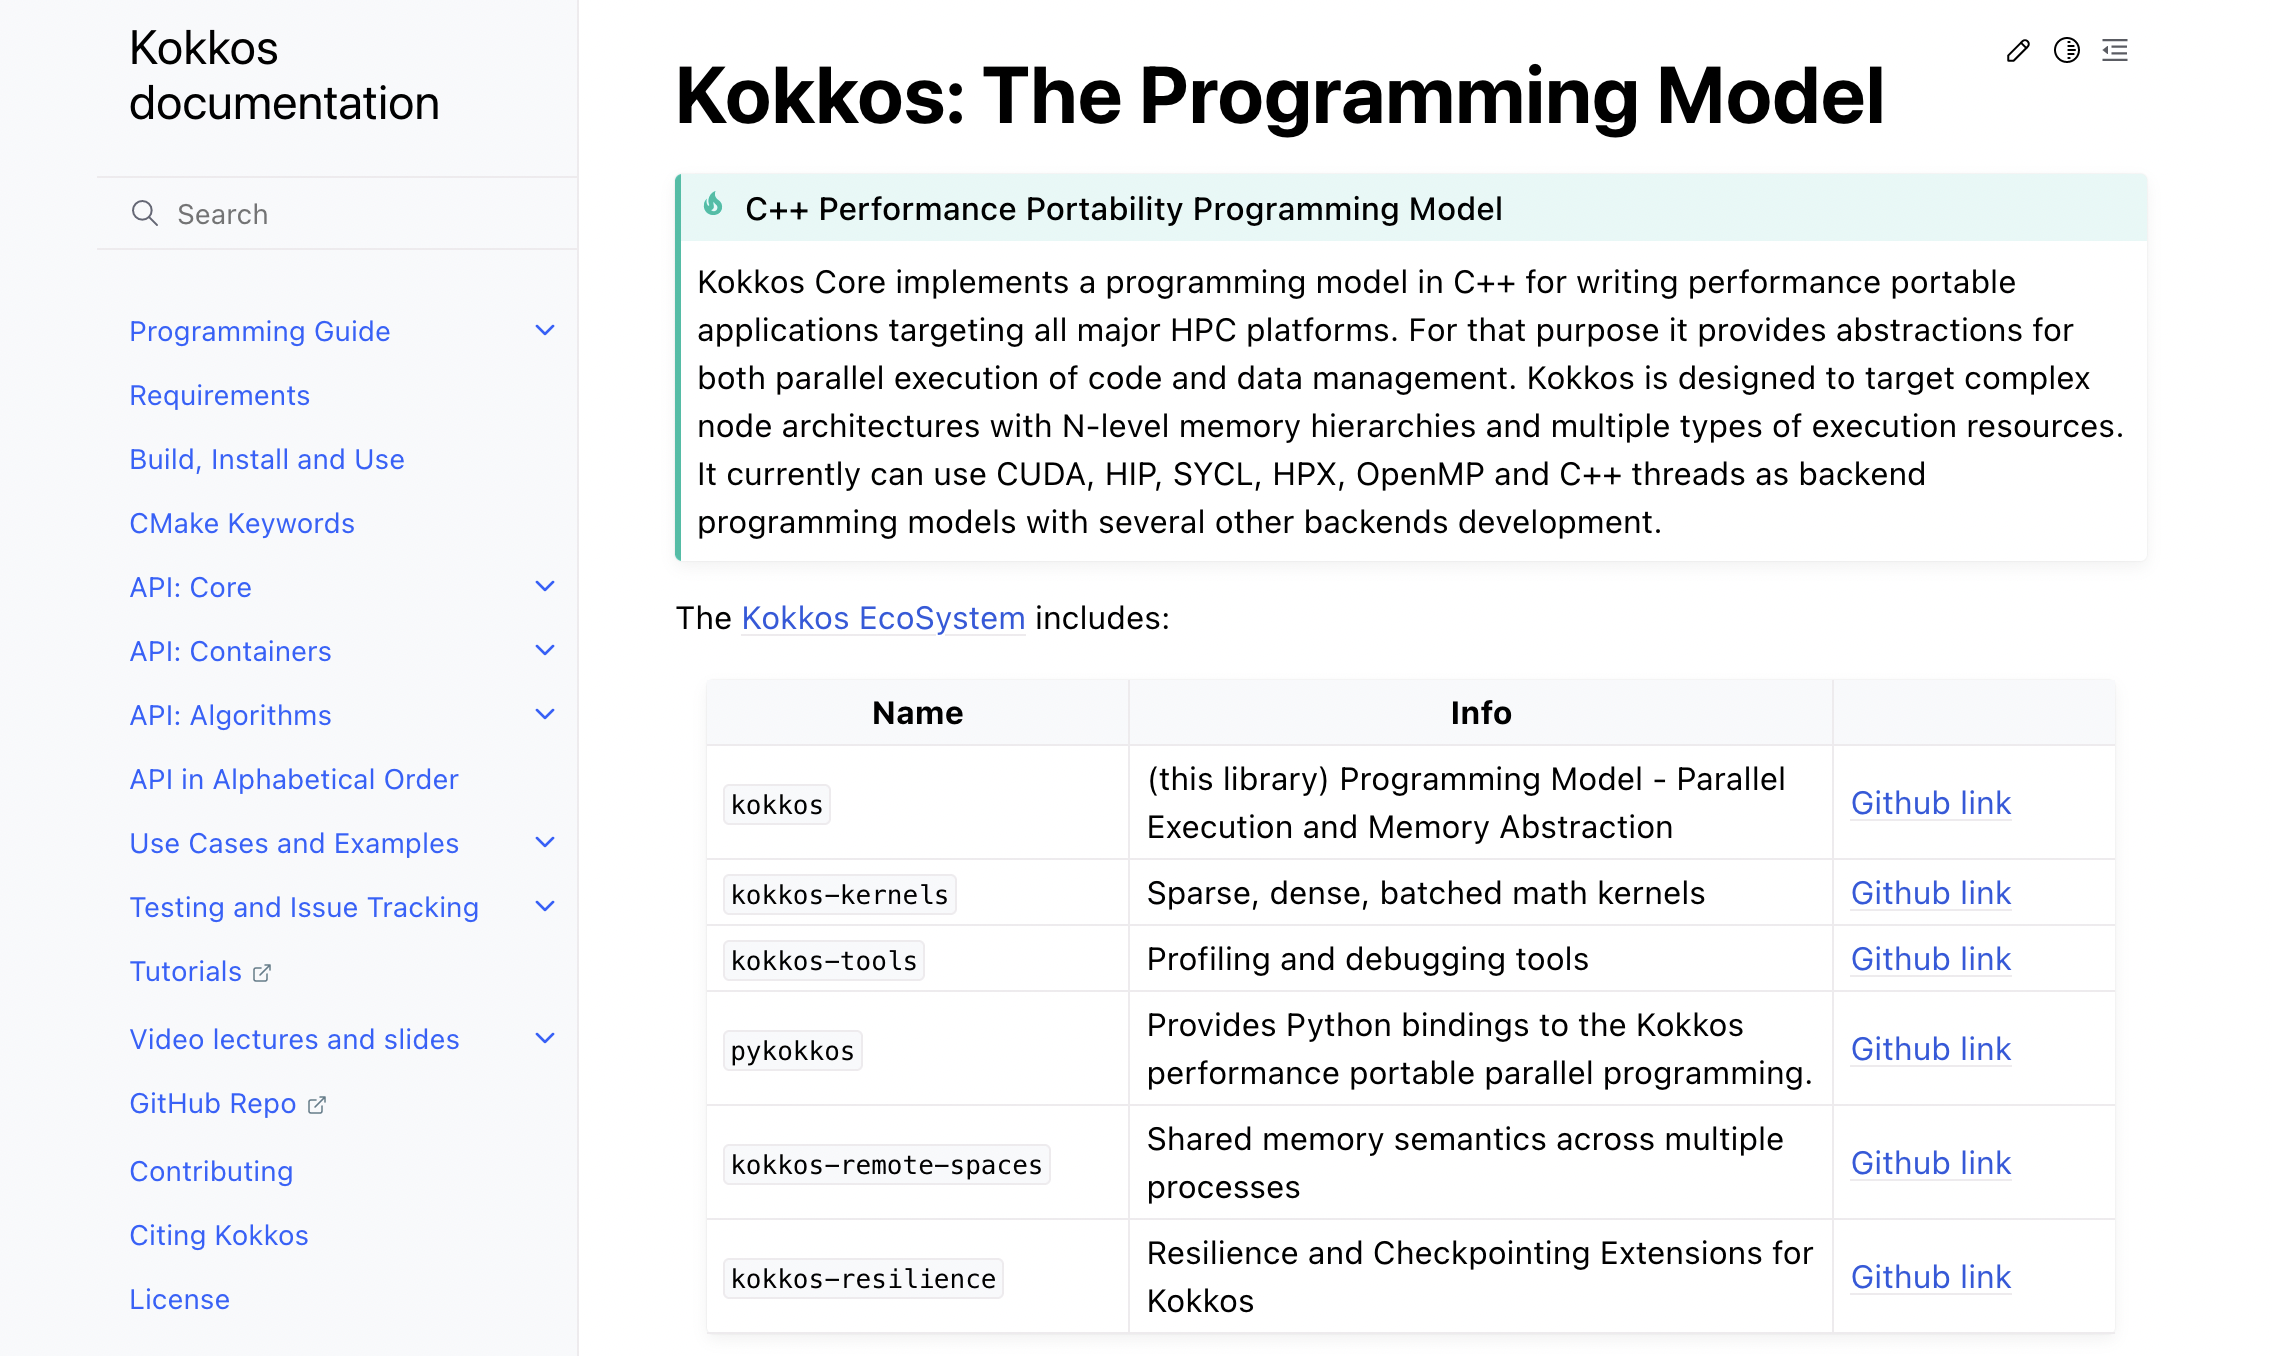
\includegraphics[width=0.9\textwidth]{3_7/website.png}
\end{frame}

\begin{frame}[fragile]{Good to know}
\textbf{Math functions are now in the primary namespace}
\begin{itemize}
  \item Now call \texttt{Kokkos::sin} etc. instead of \texttt{Kokkos::Experimental::sin}
\end{itemize}

\vspace{20pt}
\textbf{Enabled nested reduce with teams that are not power-of-two size!} 

\end{frame}
